% WACV 2024 Paper Template
% based on the CVPR 2023 template (https://media.icml.cc/Conferences/CVPR2023/cvpr2023-author_kit-v1_1-1.zip) with 2-track changes from the WACV 2023 template (https://github.com/wacv-pcs/WACV-2023-Author-Kit)
% based on the CVPR template provided by Ming-Ming Cheng (https://github.com/MCG-NKU/CVPR_Template)
% modified and extended by Stefan Roth (stefan.roth@NOSPAMtu-darmstadt.de)

\documentclass[10pt,twocolumn,letterpaper]{article}

%%%%%%%%% PAPER TYPE  - PLEASE UPDATE FOR FINAL VERSION
\usepackage[T1]{fontenc}    % use 8-bit T1 fonts
%\usepackage[review,algorithms]{wacv}      % To produce the REVIEW version for the algorithms track
%\usepackage[review,applications]{wacv}      % To produce the REVIEW version for the applications track
\usepackage{wacv}              % To produce the CAMERA-READY version
%\usepackage[pagenumbers]{wacv} % To force page numbers, e.g. for an arXiv version


% It is strongly recommended to use hyperref, especially for the review version.
% hyperref with option pagebackref eases the reviewers' job.
% Please disable hyperref *only* if you encounter grave issues, e.g. with the
% file validation for the camera-ready version.
%
% If you comment hyperref and then uncomment it, you should delete
% ReviewTempalte.aux before re-running LaTeX.
% (Or just hit 'q' on the first LaTeX run, let it finish, and you
%  should be clear).
\usepackage[pagebackref,breaklinks,colorlinks]{hyperref}


% Include other packages here, before hyperref.
\usepackage{graphicx}
\usepackage{amsmath}
\usepackage{amssymb}
\usepackage{booktabs}


\usepackage{url}            % simple URL typesetting
\usepackage{amsfonts}       % blackboard math symbols
\usepackage{nicefrac}       % compact symbols for 1/2, etc.
\usepackage{microtype}      % microtypography
\usepackage{lipsum}         % Can be removed after putting your text content
\usepackage[numbers]{natbib}
\usepackage{doi}

%% extra
\usepackage{listings}
\usepackage{amsmath} 
\usepackage{xcolor}

% Support for easy cross-referencing
\usepackage[capitalize]{cleveref}
\crefname{section}{Sec.}{Secs.}
\Crefname{section}{Section}{Sections}
\Crefname{table}{Table}{Tables}
\crefname{table}{Tab.}{Tabs.}


%%%%%%%%% PAPER ID  - PLEASE UPDATE
\def\wacvPaperID{*****} % *** Enter the WACV Paper ID here
\def\confName{WACV}
\def\confYear{2024}


\begin{document}

\title{ShitSpotter --- A Dog Poop Detection Algorithm and Dataset}

\author{Jonathan Crall\\
Kitware\\
{\tt\small jon.crall@kitware.com}
%{\tt\small erotemic@gmail.com}
% For a paper whose authors are all at the same institution,
% omit the following lines up until the closing ``}''.
% Additional authors and addresses can be added with ``\and'',
% just like the second author.
% To save space, use either the email address or home page, not both
%\and
%Second Author\\
%Institution2\\
%First line of institution2 address\\
%{\tt\small secondauthor@i2.org}
}
\maketitle

%%%%%%%%% ABSTRACT
\begin{abstract}

%This work chronicles one researcher's un-funded journey to build a phone
%application that can detect dog poop in images, and make the data widely
%available as a benchmark dataset.
We introduce a new --- currently 42GB --- "living" dataset of phone images of
dog poop with manually traced or adjusted polygon labels.
The collection and annotation of this data started in late 2020 and is planned
to continue indefinitely.

The most recent snapshot of dataset is made publicly available across three
different distribution methods: one centralized and two decentralized (IPFS and
BitTorrent).
We perform an analysis and experimental comparison of the trade-offs between
distribution methods and discuss the feasibility of each with respect to
sharing open scientific data.

A baseline vision transformer is trained to segment the objects of interest
under a grid of hyperparameters, and we evaluate their impact. The best model
achieves a pixelwise mean average precision of ~0.8ish. 
Model weights are made publicly available with the dataset. 

Code to reproduce experiments is hosted on GitHub.

%A phone application to detect poop with these models is being developed and 
%will be made freely available.

\end{abstract}

%%%%%%%%% BODY TEXT
\section{Introduction}
\label{sec:intro}

Applications of a computer vision system able to detect and localize poop in
images are numerous.
Automated waste disposal to keep parks and backyards clean.
A part of a system for using feces to monitor wildlife populations.
A warning system in smart-glasses to prevent people from stepping in poop.
Simply helping a dog owner find their dog's poop in a leafy park so they can pick it up.
Many of these applications can be realized with modern object detection and
segmentation methods (cite modern object detection and segmentation methods)
and a large labeled dataset to train on.

Poop detection is also a simple problem with a narrower scope (just a single
class), suitable for exploring the capabilities of object detection models that
focus on a single labeled class while also containing non-trivial challenges.


\begin{figure}[h]
\centering
\includegraphics[height=200pt]{/data/joncrall/dvc-repos/shitspotter_dvc/analysis/viz_three_images.jpg}
\caption[]{
    The "before/after/negative" process.
}
\label{fig:AllPolygons}
\end{figure}

There are several challenges in detecting dog poop in phone-camera images:
resolution (quality of camera, distance to the camera),
distractors,
occlusion,
variation in appearance (old/new/healthy/sick).

Towards these ends we introduce a dataset suitable for training poop detection
models in order to enable applications that require detecting or localizing
poop in images. \Cref{fig:AllPolygons}.

Discuss building the dataset

Discuss building the segmentation models

For a dataset to be of scientific use it must be accessible. 

Centralized methods are the typical choice and offer very good speeds, 
but they requires an institution willing to host or payment for a hosting service,
can prone to outages (give VGG outage as example),
and version control is not built in.

Decentralized methods allow volunteers to host data offers ability to validate
data integrity. This motivates us to compare and contrast Cloud Services,
BitTorrent, and IPFS as mechanisms for distributing datasets.


Our contributions are:
1. A challenging new \textbf{open dataset} of images with polygon segmentations.
2. An experimental \textbf{evaluation of baseline training} methods.
3. An experimental \textbf{comparison of dataset distribution} methods.
4. \textbf{Open code and models}.
Related work is discussed at the end.

% https://gist.github.com/liamzebedee/4be7d3a551c6cddb24a279c4621db74c
% https://gist.github.com/liamzebedee/224494052fb6037d07a4293ceca9d6e7


\section{Dataset}

Our first contribution is the collection of a new open dataset consisting of
dog poop images in a mostly urban environment and primary from three specific
dogs. Indoor images and poop from other dogs are present in the dataset but
were encountered less often and thus are less frequent.

The majority of the dataset was collected using the "before/after/negative"
protocol.
When we encountered a poop in the wild --- usually from our own dogs, but
sometimes from other dogs --- before we dispose of it we 
take a "before" picture containing the poop.
Then we pick up the poop and take an "after" picture of the same area. 
Then we find a nearby area or perhaps something else in the nearby environment
that might act as a confuser (e.g. pine cone or leaf) and take a third
"negative" picture.

The majority of images in the dataset follow this pattern. However, there are exceptions.
The first 6 months of data collection only involved the "before/after" part of the protocol.
Sometimes the researcher failed or was unable to take the 2nd or 3rd image.


Only roughly 1/3 of the dataset has annotations due to the other 2/3 of the
images being taken in a way where the object of interest was removed from the
scene.

There are some cases where the before / after / negative protocol was not followed, but this can be identified.

Additionally, the dataset also contains a few dozen (84ish) images contributed
by friends and family. These images are images largely do not follow the
before/after protocol and are marked for use only in testing.


\begin{figure}[h]
\centering
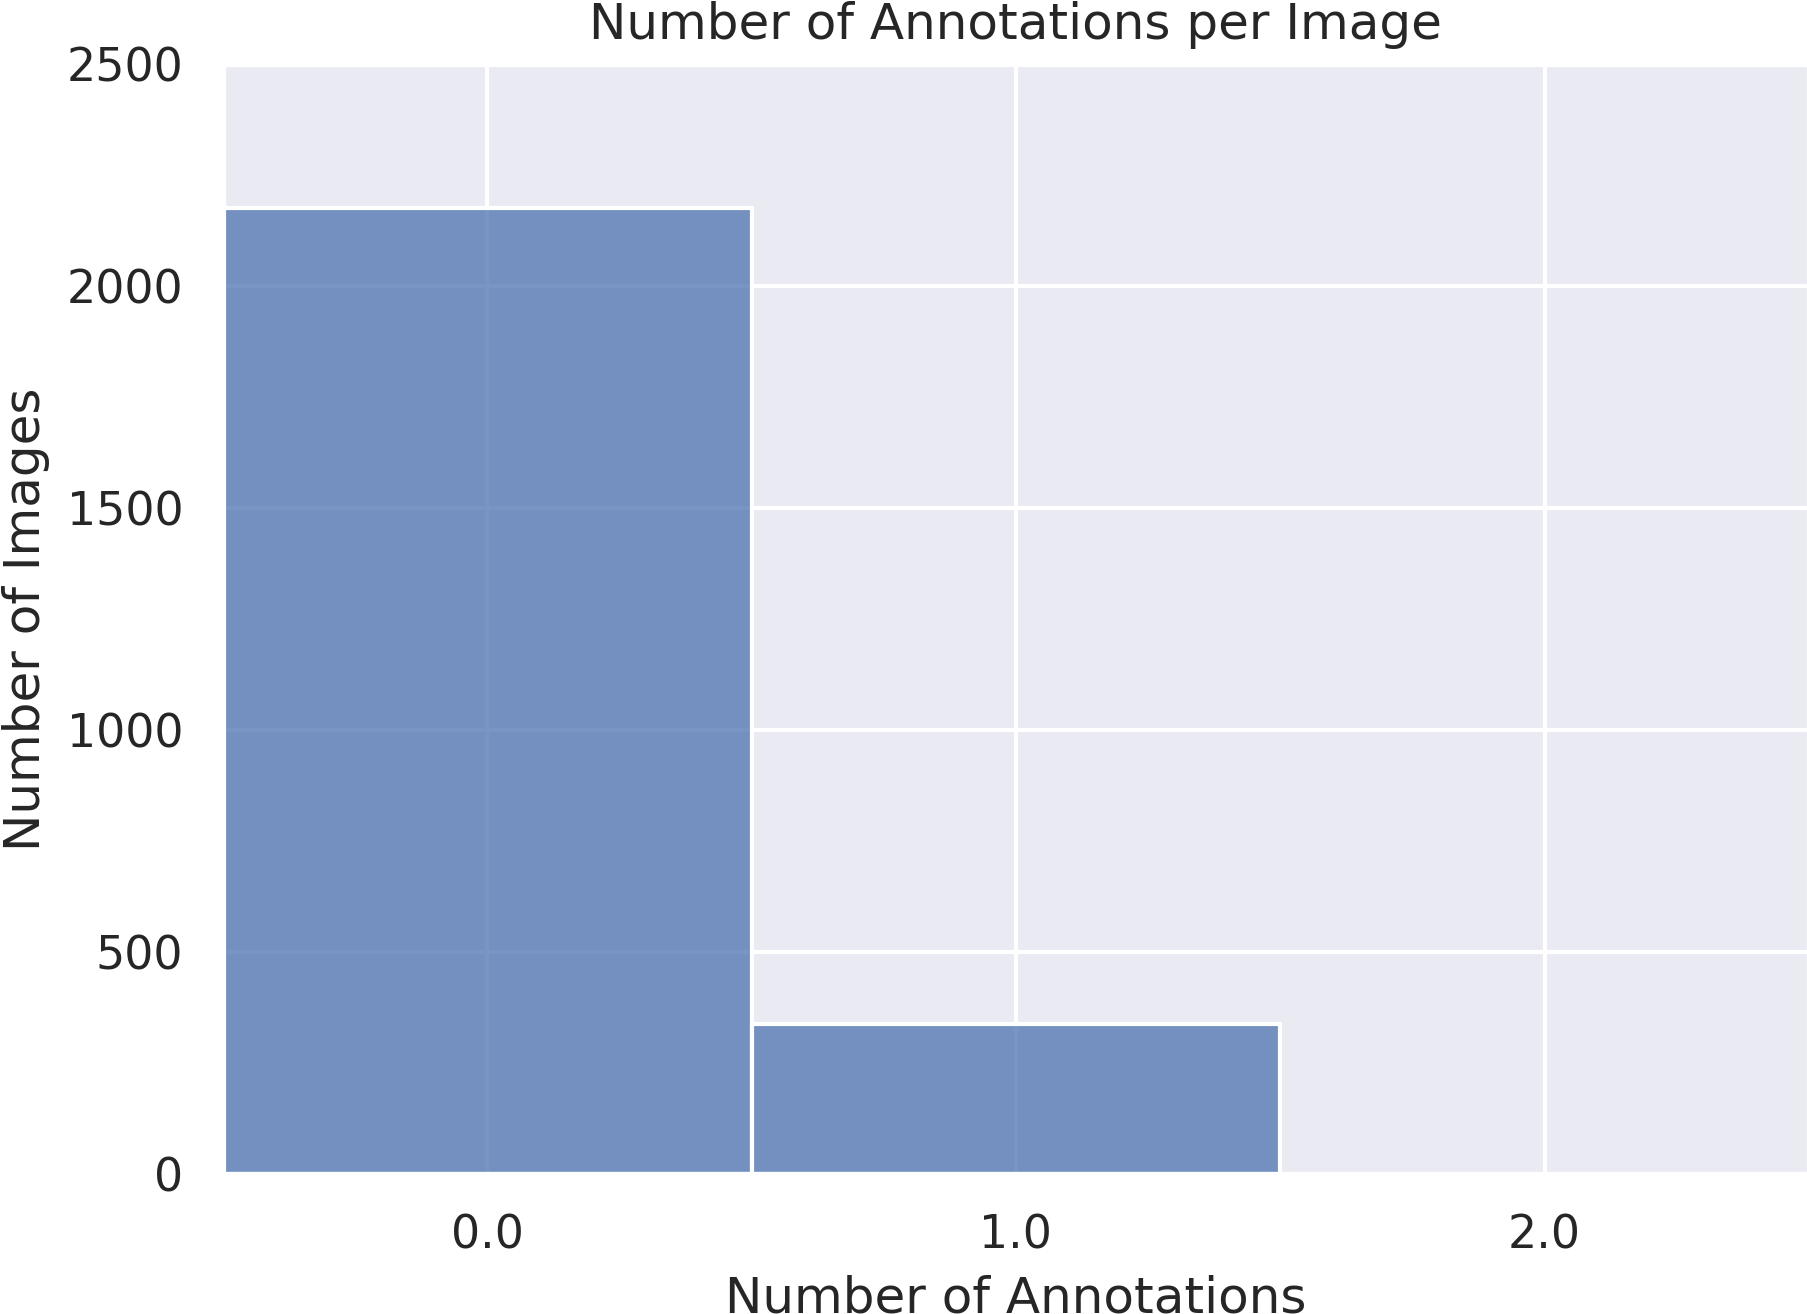
\includegraphics[height=160pt]{/home/joncrall/code/shitspotter/coco_annot_stats/annot_stat_plots/anns_per_image_histogram.png}
\caption[]{
    Histogram of the number of annotations per image. 
    Only 35\% (2346) of the images contain annotations, the other 65\% (4302)
    are known not to contain poop. Of these 4302 about half of them were taken
    directly after the poop was picked up, and the other half are pictures of a
    nearby location. 
}
\label{fig:AnnotsPerImage}
\end{figure}


% https://arxiv.org/abs/1803.09010
Data is released with a datasheet describing its characteristics \cite{gebru_datasheets_2021}.

Challenges

\paragraph{Construction}

Labelme \cite{wada_labelmeailabelme_nodate} for annotations with segment anything \cite{kirillov_segment_2023}.
The boundaries of all annotated polygons are illustrated in \Cref{fig:AllPolygons}.

Anecdotal note: SAM \cite{kirillov_segment_2023} worked well to automatically
segment the poop, many of these needed adjustments, especially in regions of
shadows, but there were cases that required a completely manual approach.
Unfortunately a clean record of what cases these were does not exist. 

% python -m shitspotter.cli.coco_annotation_stats $HOME/data/dvc-repos/shitspotter_dvc/data.kwcoco.json

\begin{figure}[h]
\centering
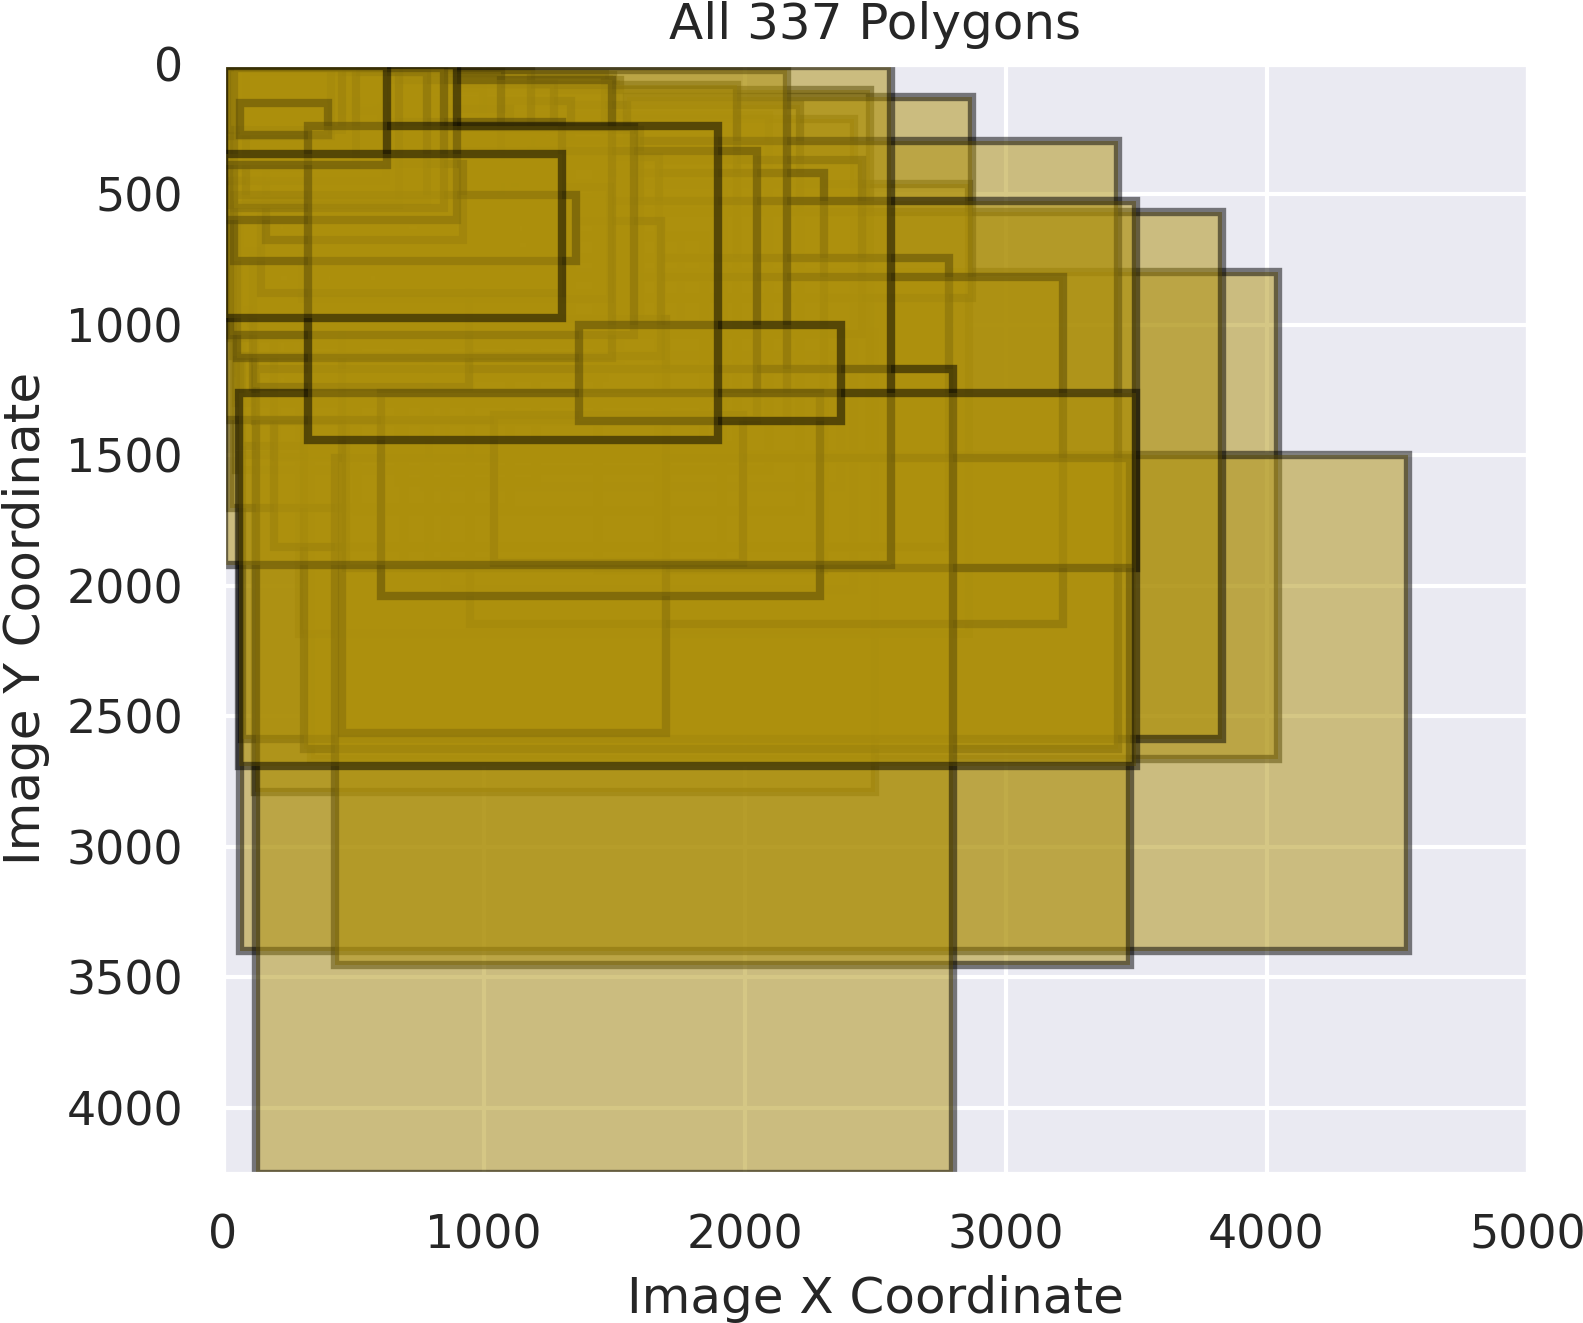
\includegraphics[height=230pt]{/home/joncrall/code/shitspotter/coco_annot_stats/annot_stat_plots/all_polygons.png}
\caption[]{
    All annotations drawn on a single images with 0.8 opacity to demonstrate
    the distribution in annotation location, shape, and size with respect to
    image coordinates.
}
\label{fig:AllPolygons}
\end{figure}

\paragraph{Analysis}

Number of images, annotations, and other stats.


\section{Models}

Our second contribution is an evaluation of several trained models to serve as
a baseline.

We use the training and evaluation system of \cite{Greenwell_2024_WACV}, which
can be trained to predict heatmaps from polygons and can evaluate those
heatmaps on a pixelwise-level. 

The baseline architecture is a variant of a vision-transformer \cite{vit,split-attention,greenwell_watch_2024}.

Number of parameters.
Memory at train time.
Memory at predict time.
Model size on disk.

We train several models and vary the learning rate, weight decay,
shrink-and-perterb regularization \cite{ash_warm_starting_2020}, as well as
other ad hoc experiment settings.
%\textbf{Static Parameters}:

\subsection{Model Experiments}

After finding a reasonable performing starting point, we performed an ablation
over learning rate and regularization parameters. 

This restricted set is illustrated in \Cref{fig:scatter-subset}.

We evaluate each model with standard pixelwise segmentation metrics with a
focus on average-precision (AP) and  area under the ROC curve (AUC)
\cite{metrics} .

\Cref{fig:scatter-all} illustrates the AP and AUC of all baseline models trained.
These include ad-hoc parameters settings when searching for a stable training
configuration.

The resources used are given in \Cref{fig:resource}.

\section{Distribution}

% BitTorrent can be vulnerable to MITM:
% https://www.reddit.com/r/technology/comments/1dpinuw/south_korean_telecom_company_attacks_torrent/

Our third contribution is an exploration of distributed and centralized data distribution methods. 

Cloud storage for a modest amount of data can be expensive.

Decentralized methods can allow information to persist so long as at least 1
person has the data.

BitTorrent is a well known distributed system.

IPFS is a new similar tool.


Discuss distributing the dataset via IPFS versus centralized distribution
systems.

Decentralized Method - IPFS and BitTorrent.
Centralized Method - Girder

Observations:
\begin{itemize}
    \item IPFS via https using gateways does not always work well.
    \item IPFS usually works well if you use the CLI.
    \item IPFS is easier to update.
    \item IPFS does rehash every file, which induces an O(N) scalability constraint.
    \item IPFS does rehash every file, which induces an O(N) scalability constraint.
\end{itemize}


IPFS vs BitTorrent:

Both of which have the ability to use the Kademlia - distributed hash table (DHT) \cite{maymounkov_kademlia_2002}.
IPFS always uses its DHT, where as BitTorrent the Kademlia-based Mainline
Tracker can be disabled in favor of 3rd party trackers.

An excellent overview of protocols details can be found \cite{zebedee_comparing_2023}.
Our comparison is going to focus on measurements.

% Much of the 
% https://gist.github.com/liamzebedee/224494052fb6037d07a4293ceca9d6e7

%[Steiner, En-Najjary, Biersack 2022]

The Mainline Tracker is a DHT for bittorrent.

% See Also:
% Long Term Study of Peer Behavior in the KAD DHT
% https://git.gnunet.org/bibliography.git/plain/docs/Long_Term_Study_of_Peer_Behavior_in_the_kad_DHT.pdf
% We have been crawling the entire KAD network once a day for more than a year to track end-users with static
% IP addresses, which allows us to estimate end-user lifetime and the fraction of end-users changing their KAD ID.


% https://academictorrents.com/docs/about.html
Dataset (is / will be) tracked on Academic Torrents \cite{academic_torrents_Cohen2014}.


\subsection{Distribution Experiments}

Measure the performance of our algorithm versus a baseline.

Measure the speed of IPFS vs BitTorrent.

Time to create torrent vs time to pin to IPFS.

%-------------------------------------------------------------------------
\section{Related Work}

Object detection

Waste detection is an important problem but with relatively few open datasets.
%  https://paperswithcode.com/dataset/zerowaste
The ZeroWaste dataset \cite{bashkirova_zerowaste_2022} contains 1,800 segmented
video frames and 6000 unlabeled frames in a recycling facility.
% https://paperswithcode.com/dataset/taco
The TACO dataset \cite{proenca_taco_2020} is another "living" dataset
containing 1500 images with 4,784 annotations over 60 classes.
% TrashCan https://paperswithcode.com/dataset/trashcan
% Top Datasets on paperwith code
% https://paperswithcode.com/datasets?mod=images&task=semantic-segmentation&page=2


While ours is the largest publicly available poop dataset that we are aware of,
it is not the first.
A dataset of 100 dog poop images was collected and used to train a FasterRCNN
model in 2019 but this dataset and model are not publicly available \cite{neeraj_madan_dog_2019}.
The MSHIT dataset \cite{mshit_2020} consists of 3.89GB of real images with fake
poop (e.g. plastic poop) in controlled environments.
The company iRobot has a dataset of annotated indoor poop images used to train
Roomba j7+ to avoid collisions, but as far as we are aware, this is not
available \cite{roomba_2021}.

\section{Conclusion}

The ShitSpotter dataset is 42GB of images with polygon segmentations of dog
poop. 

We train and evaluate several baseline segmentation models, the best of which 
achieve an AP/AUC of ...

Our dataset is sufficient to train an object detection network to (level of
precision/recall).

We make data and models available over 3 distribution mechanisms: 
cloud storage, BitTorrent, and IPFS.

Decentralized methods are feasible methods of distribution, with strong
security but they can be slow.
IPFS is a promising solution for hosting scientific datasets, but does have pain points.
In contrast bittorrent can do X/Y/Z, but ...
Lastly centralized cloud storage can give the best speeds, but sacrifices some
security and can be less robust.

Directions for future research / development are:
1. Add lightweight object-level head and test object detection metrics.
2. Optimize model architectures for mobile devices.
3. Launch phone application.
4. Improve model / data distribution.


%%%%%%%%% REFERENCES
{\small
\bibliographystyle{ieee_fullname}
\bibliography{citations}
}
%\bibliographystyle{unsrtnat}
%\bibliography{references}  %%% Uncomment this line and comment out the ``thebibliography'' section below to use the external .bib file (using bibtex) .

\end{document}
